\subsection{Fullerenes}





The options to define the input parameters for the construction of the fullerene are displayed in the \textbf{Calculations--$>$Input} options:

 \begin{figure}[h!]
\centering
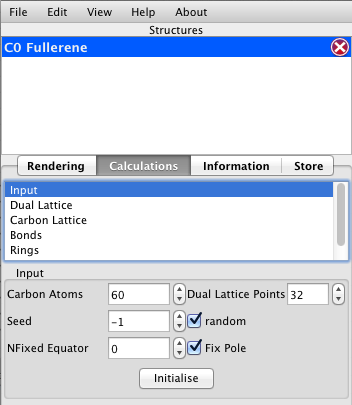
\includegraphics[scale= 0.6]{../../../../screens/nanocap_fullerene_input_win.png}
\caption{\nanocap~input options for a fullerene}
\label{fullerene_input_options}
\end{figure}

Here you can set the options for:
\begin{itemize}
 \item the number of dual lattice points or carbon atoms
 \item the seed for the initial random arrangement of dual lattice points
 \item the number of dual lattice points to hold fixed at either the poles or the equator
 \end{itemize}
 
Upon on clicking \textit{Initialise} the dual lattice points belonging to the fullerene will be constructed via the following:
\begin{equation}
\begin{array}{lcl}
x_i & = & \sqrt{1 - z_0}\cos(t_0) \\
y_i & = & \sqrt{1 - z_0}\sin(t_0) \\
z_i & = & z_0
\end{array}
\label{randomspheregen}
\end{equation}
where  $z_0$ and  $t_0$ are two random numbers in the range [$-$1,1] and [0,2$\pi$]. To visualise these points check the options outlined in Section \ref{Rendering}. The process of optimisation of these points is described in Section \ref{Optimisation}
